\begin{center}
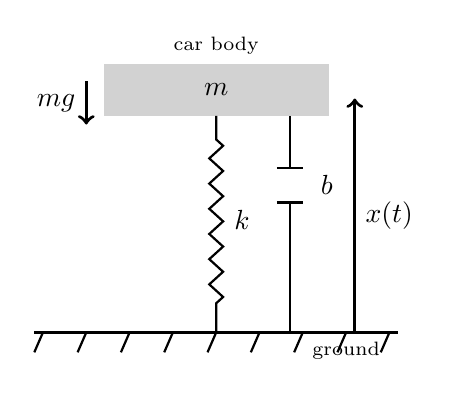
\begin{tikzpicture}[
    scale=1.1,
    spring/.style={thick, decorate, decoration={zigzag, pre length=0.3cm, post length=0.3cm, segment length=0.32cm}},
]
  % ---- car body (mass) ----
  \fill[gray!35] (-1.3,3.2) rectangle (1.3,3.8);
  \node at (0,3.5) {$m$};
  \node[font=\scriptsize, above] at (0,3.8) {car body};

  % ---- suspension: spring (left) and damper (right), in parallel ----
  \draw[spring] (0,3.2) -- (0,0.7);
  \node[right=3pt] at (0,2.0) {$k$};
  \draw[thick] (0.85,3.2) -- (0.85,2.6);
  \draw[thick] (0.70,2.6) -- (1.00,2.6);
  \draw[thick] (0.70,2.2) -- (1.00,2.2);
  \draw[thick] (0.85,2.2) -- (0.85,0.7);
  \node[right=3pt] at (1.00,2.4) {$b$};

  % ---- ground ----
  \draw[very thick] (-2.1,0.7) -- (2.1,0.7);
  \foreach \i in {0,...,8} { \draw[thick] (-2.0+0.5*\i,0.7) -- (-2.1+0.5*\i,0.47); }
  \node[font=\scriptsize, below] at (1.5,0.7) {ground};

  % ---- displacement and force arrows ----
  \draw[->, very thick] (1.6,0.7) -- (1.6,3.4) node[midway,right] {$x(t)$};
  \draw[->, very thick] (-1.5,3.6) -- (-1.5,3.1) node[midway,left] {$mg$};
\end{tikzpicture}
\end{center}
